\subsection{Simulations using GR signals in Gaussian noise} \label{ssec:gr_signal}

We now demonstrate our method using synthetic-signal injections describing GWs
from BBHs in GR. We employ coloured Gaussian noise with PSDs for LIGO and
Virgo detectors during the fourth observing (O4) run (i.e., at design sensitivity), which 
is expected to start yin the second half of 2022~\cite{AdvLIGOPSD,TheVirgo:2014hva}.
For the mock BBH signals, we choose parameters similar to two specific GW events, GW150914~\cite{Abbott:2016blz} and
GW190521~\cite{Abbott:2020tfl}. We list them in Table~\ref{tab:injection_values}.
These two binary systems are representative of the kind of systems for which
the QNM measurement is most suitable, notably high-mass BBH events which are loud enough that the
pre- and post-merger SNRs return reliable parameter-estimation results.

%%%%%%%%%%%%%%%%%%%%%%%%%%%%%%%%%%%%%%%%%%%%%%%%%%%%%%%%%%%%%%%
% Table for Injections
%%%%%%%%%%%%%%%%%%%%%%%%%%%%%%%%%%%%%%%%%%%%%%%%%%%%%%%%%%%%%%%
\begin{table}[h!]
\begin{center}
\begin{tabular}{ c|c|c|c|c|c|c|c|c }

Injection &  Network & \makecell{$m_{\rm 1\,det}$ \\$(\Mo)$} &  \makecell{$m_{\rm 2\,det}$ \\ $(\Mo)$} & $\chi_{1}$ & $\chi_{2}$ & $\rho_\text{IMR}$ & $\rho_\text{insp}$ & $\rho_\text{postinsp}$ \\
 \hline
 GW150914-like & HL &39 & 31 & 0.0 & 0.0 & 25 & 22 & 12 \\
 GW190521-like & HL & 150 & 120 & 0.02 & -0.39 & 20 & 8 & 18 \\
 SXS:BBH:0166 & HLV &72 & 12  & 0.0 & 0.0 & 71 & 58 & 41 \\

\end{tabular}
\caption{Parameters of the synthetic-signal injections, chosen to be similar to the actual GW events indicated in the first column (first two rows). The parameters $(m_{\rm 1 \,det}, m_{\rm 2 \,det})$ are the detector-frame masses of the primary and secondary BHs, respectively. The third row indicates the parameters of the SXS BBH waveform used in Sec.~\ref{ssec:nohairtheorem}. The second column refers to the detector-network used, with H,L,V, referring to LIGO-Hanford, LIGO-Livingston and Virgo, respectively. The quantities $\rho_\text{IMR}$, $\rho_\text{insp}$ and $\rho_\text{postinsp}$ are the SNR of the full IMR signal, SNR upto a certain cutoff frequency, and SNR after the cutoff frequency respectively. In each case, the cutoff frequency is assumed to be the frequency at the innermost circular stable orbit (ISCO) corresponding to the remnant Kerr BH.}
\label{tab:injection_values}
\end{center}
\end{table}
%%%%%%%%%%%%%%%%%%%%%%%%%%%%%%%%%%%%%%%%%%%%%%%%%%%%%%%%%%%%%%%
%%%%%%%%%%%%%%%%%%%%%%%%%%%%%%%%%%%%%%%%%%%%%%%%%%%%%%%%%%%%%%%


%%%%%%%%%%%%%%%%%%%%%%%%%%%%%%%%%%%%%%%%%%%%%%%%%%%%%%%%%%%%%%%
% Simulated siganl: GR
%%%%%%%%%%%%%%%%%%%%%%%%%%%%%%%%%%%%%%%%%%%%%%%%%%%%%%%%%%%%%%%
\begin{figure*}[hbt]
\begin{center}
        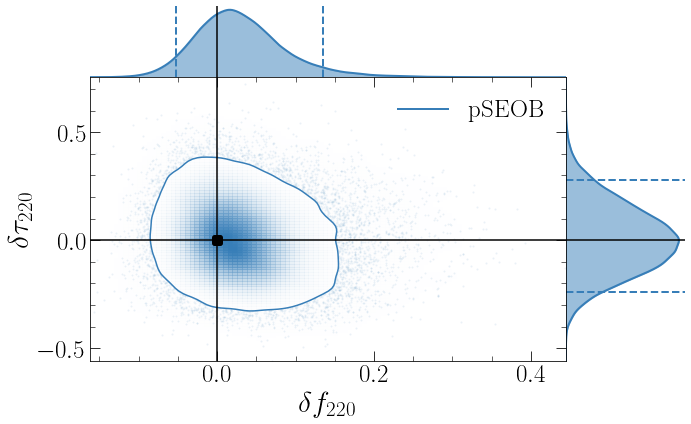
\includegraphics[width=0.5\textwidth]{figures/GW150914_simulated_signal_0p0_deltaf220_deltatau220.png}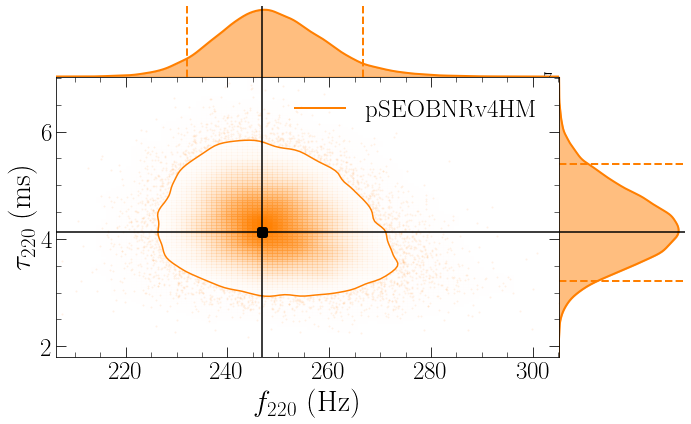
\includegraphics[width=0.5\textwidth]{figures/GW150914_simulated_signal_0p0_f220_tau220.png}
        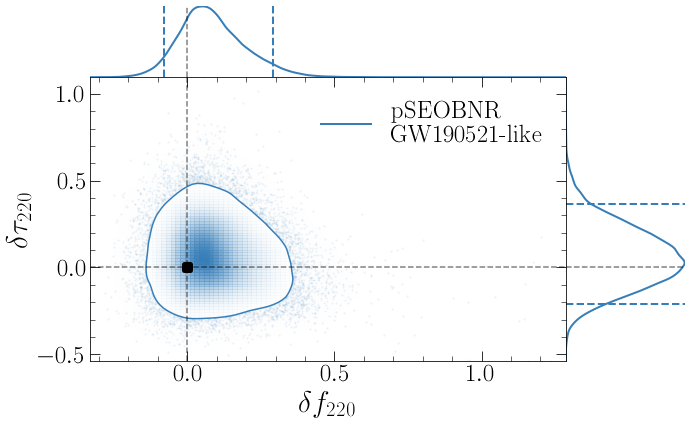
\includegraphics[width=0.5\textwidth]{figures/GW190521_simulated_signal_0p0_deltaf220_deltatau220.png}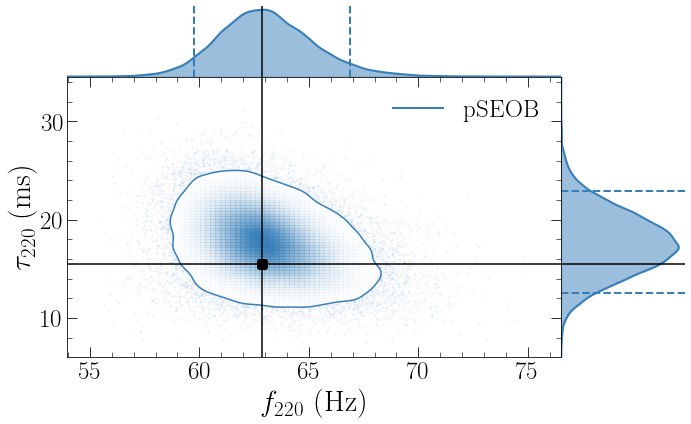
\includegraphics[width=0.5\textwidth]{figures/GW190521_simulated_signal_0p0_f220_tau220.png}
        \caption{\textcolor{red}{FINAL RESULT} Posterior probability
          distribution on the fractional deviations in the frequency
          and damping time of the $(2,2)$ QNM, $(\df{220},\dtau{220})$
          (left panels) and the reconstructed quantities,
          $(\fngr{220}, \taungr{220})$ (right panels) for GR
          injections ($\SEOB$) with initial parameters similar to GW150914 (top
          panels) and GW190521 (bottom panels)
          (see Table~\ref{tab:injection_values}). The 2D contour marks the
          90\% credible region, while the dashed lines on the 1D
          marginalized distributions mark the 90\% credible
          levels. The black vertical and horizontal lines mark the
          injection values.}
        \label{fig:simulated_signal_GR}
\end{center}
\end{figure*}
%%%%%%%%%%%%%%%%%%%%%%%%%%%%%%%%%%%%%%%%%%%%%%%%%%%%%%%%%%%%%%%
%%%%%%%%%%%%%%%%%%%%%%%%%%%%%%%%%%%%%%%%%%%%%%%%%%%%%%%%%%%%%%%

To avoid possible systematic biases in our parameter-estimation analysis
due to error in waveform modeling, we use the GR version of the same waveform,
$\SEOB$ (i.e., without allowing for deviations in the QNM parameters) to
simulate our GW signal. And to avoid systematic biases due to noise,
we use an averaged (zero-noise) realization of the noise. \footnote{A detailed
study on noise systematics for one of the GW events is presented in
Appendix~\ref{sec:noise_systematics}.}  As in the case of the actual
detections of GW150914 and GW190521, we consider a two-detector LIGO network at
Hanford and Livingston, having identical PSDs. The distance to the two 
synthetic events is rescaled such that the SNR in the detector network
is the same as the actual events (i.e., 24 for GW150914 and 14
for GW190521). Since mearly--equal-mass binaries like GW150914 and
GW190521 observed at moderately high SNRs are not expected to have a
loud ringdown signal, we restrict ourselves to estimating the
frequency and damping time of only one QNM $(\ell m) = (2,2)$ (i.e.,
$\{\df{220},\dtau{220}\}$), while fixing the other QNM frequencies to
their GR values.

We find, as one might expect, that the posterior distribution on the
parameters describing fractional deviations in the frequency and
damping time are consistent with zero (left panels of
Fig.~\ref{fig:simulated_signal_GR}). One can then convert these
fractional quantities into absolute quantities using the relations
given in Eqs.~\ref{eq:nongr_freqs_a} and ~\ref{eq:nongr_freqs_b}, and
construct posterior distributions on these effective quantities,
$(\fngr{220}, \taungr{220})$ (right panels of
Fig.~\ref{fig:simulated_signal_GR}). In each of these cases, the recovered
two-dimensional posteriors are consistent with the GR predictions
(black dashed lines).


\subsection{Simulations using non-GR signals in Gaussian noise} \label{ssec:ngr_signal}

To demonstrate the robustness of the method in detecting possible
deviations from GR, we inject synthetic GW signals which are identical to
the corresponding GR prediction up to merger, and differ in their post-merger
description. We again choose binary-parameters
similar to GW150914 and GW190521 (see Table ~\ref{tab:injection_values}), but
set $\df{220} = \dtau{220} = 0.1 $.
In other words, we assume that the frequency and damping time
of our non-GR signal is 10\% more than the corresponding GR prediction,
although the pre-merger signal is identical to GR. In Fig.~\ref{fig:nongr_waveform}
we show this non-GR waveform, \texttt{pSEOBNR} with respect to the 
original GR template, \texttt{SEOBNR}. We see that the waveforms are identical in amplitude
and instanteneous frequency upto the merger (lower panel) , beyond which the 
red (GR template) and blue (non-GR template) differ. We summarize the results of the Bayesian analysis in Fig.~\ref{fig:simulated_signal_nonGR} where we
show the posterior probability distributions for $(\df{220}, \dtau{220})$, or equivalently
$(\fngr{220}, \taungr{220})$. We find that they are consistent with the corresponding
values of the injection parameters, indicated by the black dashed lines.

%%%%%%%%%%%%%%%%%%%%%%%%%%%%%%%%%%%%%%%%%%%%%%%%%%%%%%%%%%%%%%%
%%%%%%%%%%%%%%%%%%%%%%%%%%%%%%%%%%%%%%%%%%%%%%%%%%%%%%%%%%%%%%%
\begin{figure}
        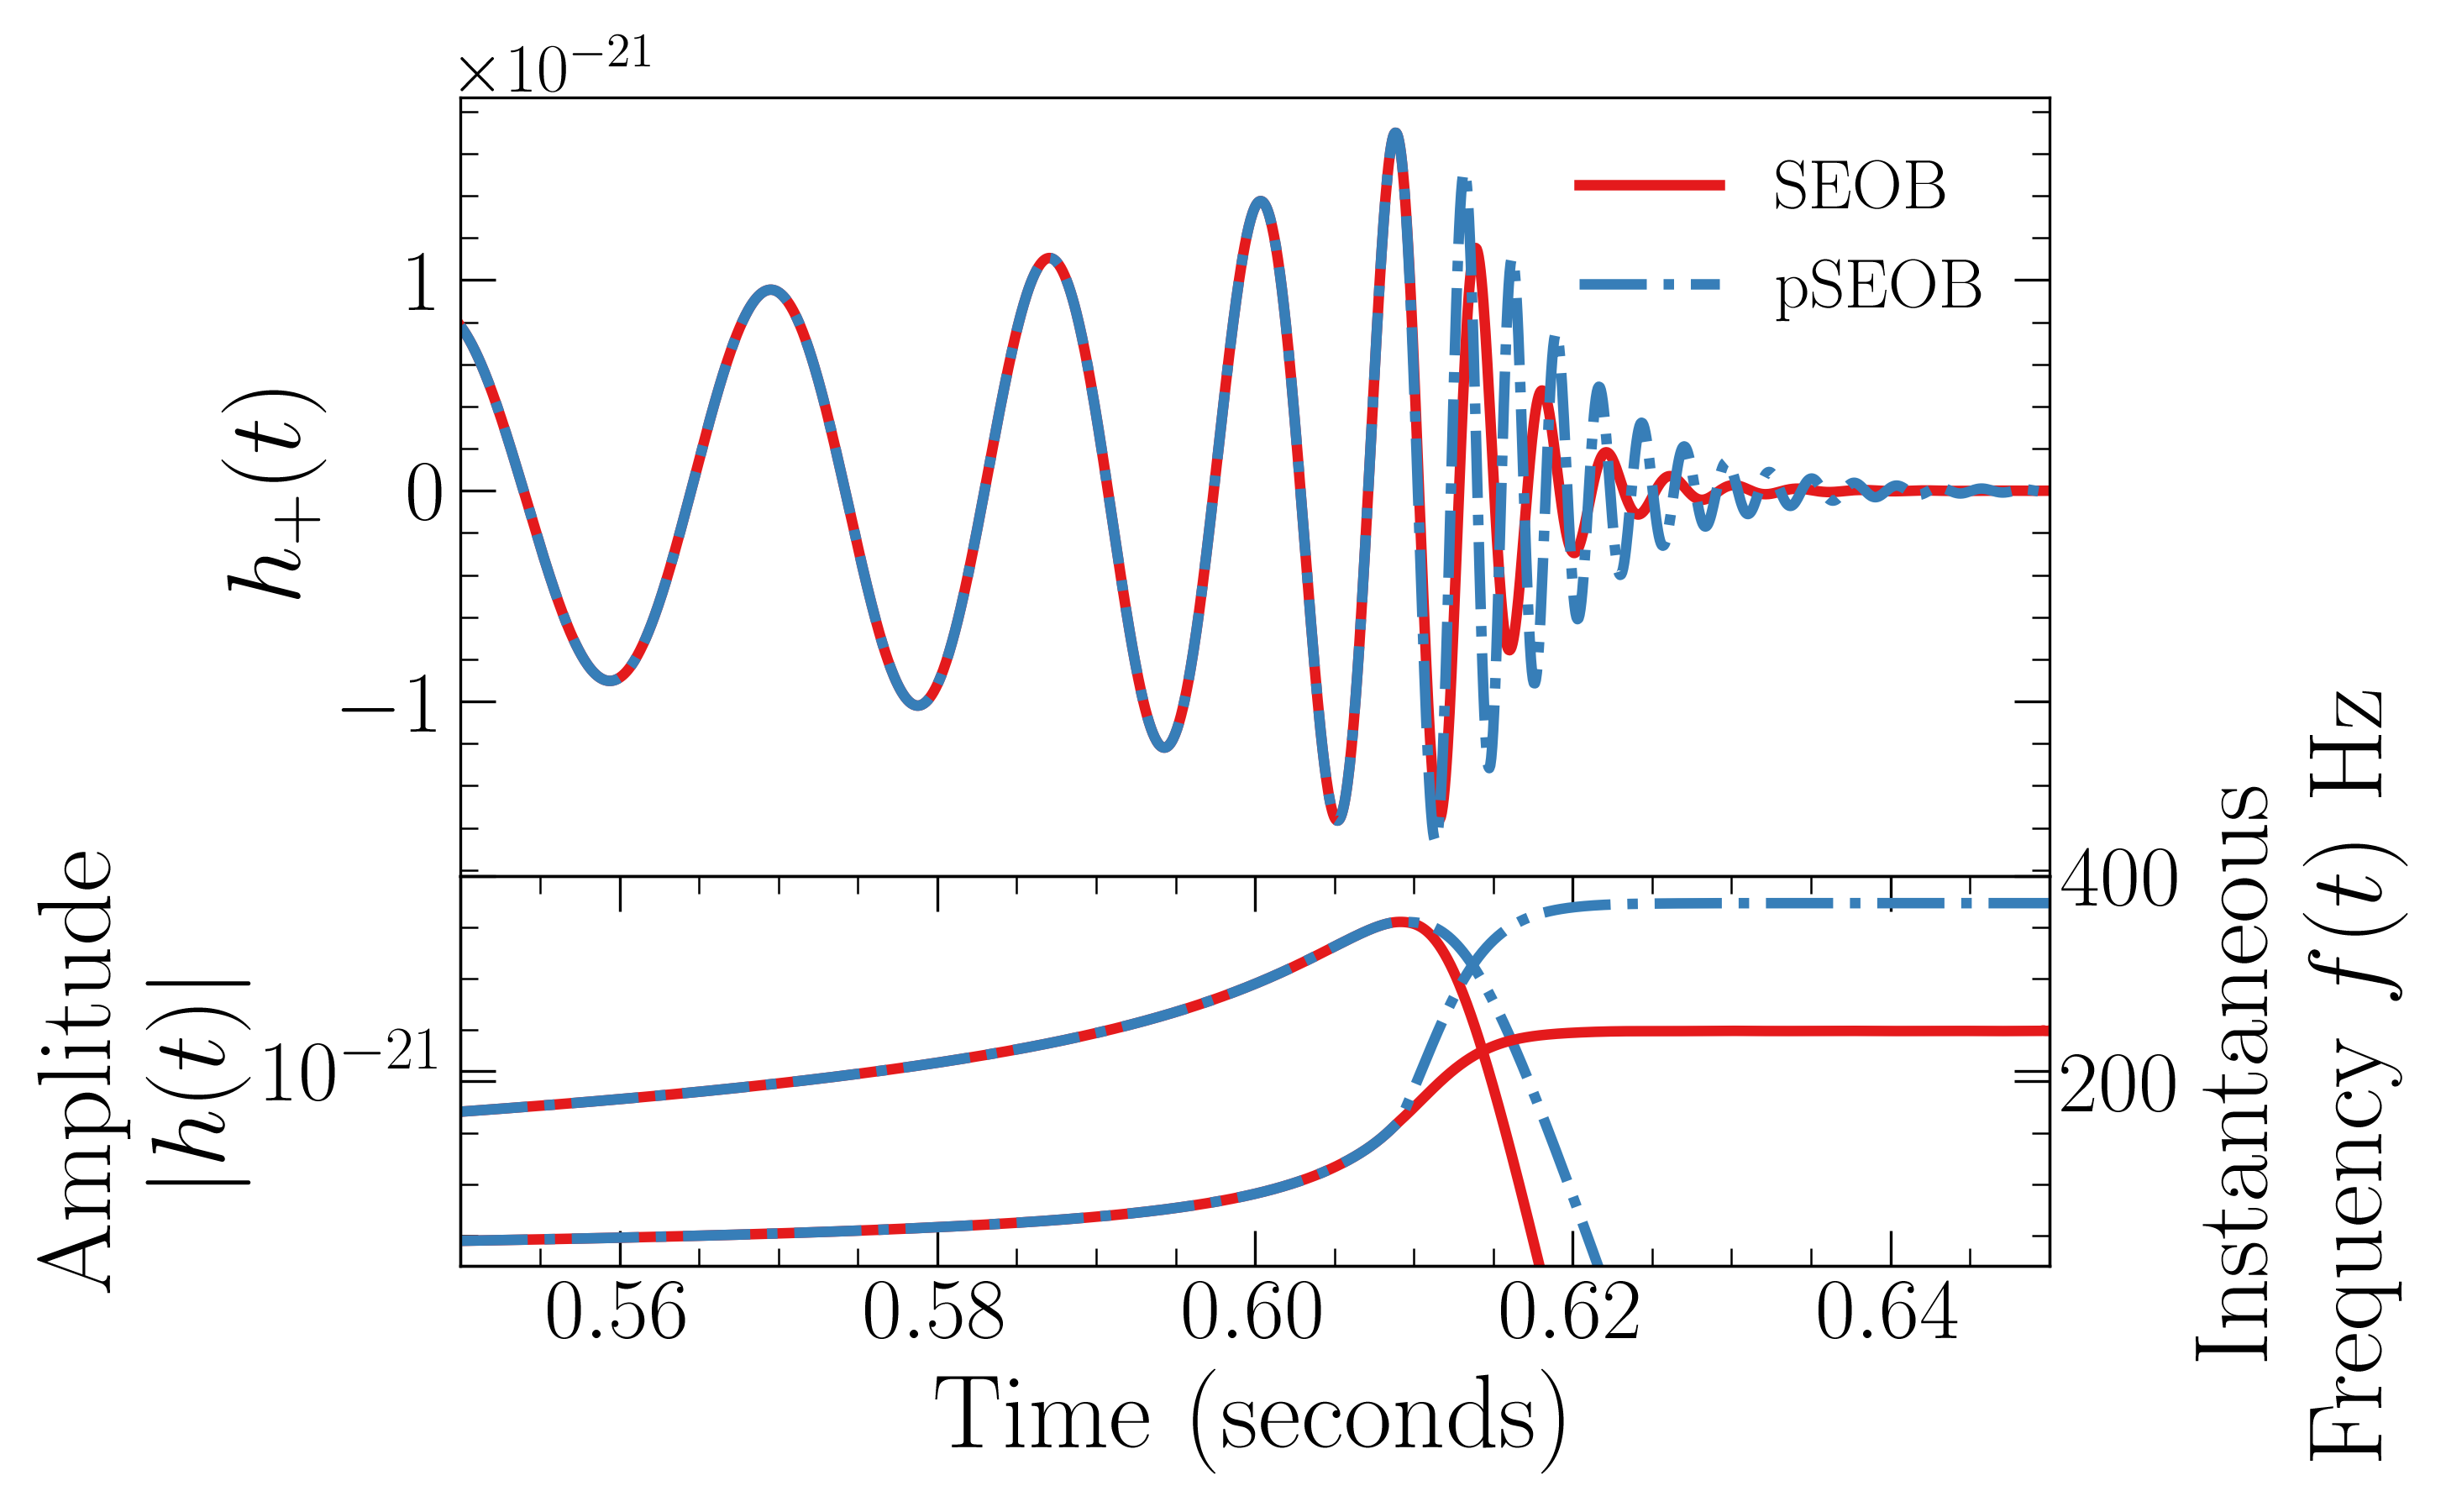
\includegraphics[width=0.5\textwidth]{figures/modGR_waveforms_amplitudephase.png}
        \caption{\textcolor{red}{FINAL RESULT} Top panel: The `+'--polarization of the gravitational waveform $h_+(t)$ from a GW150914-like event where the post-merger is described by GR (i.e., $\df{220} = \dtau{220} = 0$), and where the merger-ringdown is modified (i.e., $\df{220} = \dtau{220} = 0.1$). Bottom panel: Comparison of the evolution of the amplitude, $\tilde{h}(t)$ (left) and instantaneous frequency, $f(t)$ (right) for the GR and non-GR signal.}
        \label{fig:nongr_waveform}
\end{figure}
%%%%%%%%%%%%%%%%%%%%%%%%%%%%%%%%%%%%%%%%%%%%%%%%%%%%%%%%%%%%%%%
%%%%%%%%%%%%%%%%%%%%%%%%%%%%%%%%%%%%%%%%%%%%%%%%%%%%%%%%%%%%%%%

%%%%%%%%%%%%%%%%%%%%%%%%%%%%%%%%%%%%%%%%%%%%%%%%%%%%%%%%%%%%%%%
% Simulated siganl: non-GR
%%%%%%%%%%%%%%%%%%%%%%%%%%%%%%%%%%%%%%%%%%%%%%%%%%%%%%%%%%%%%%%
\begin{figure*}%[h!]
\begin{center}
        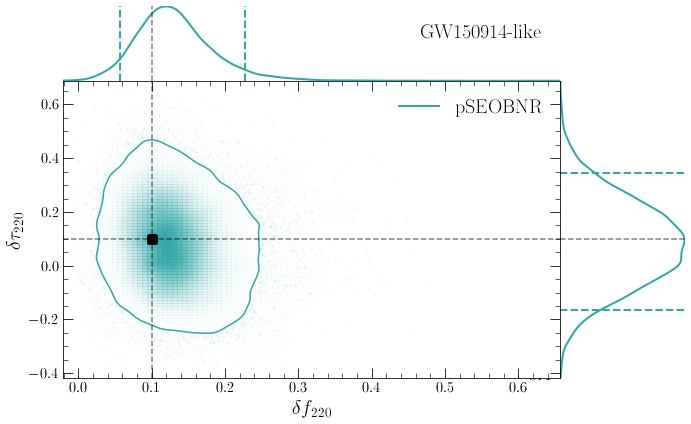
\includegraphics[width=0.5\textwidth]{figures/GW150914_simulated_signal_0p1_deltaf220_deltatau220.png}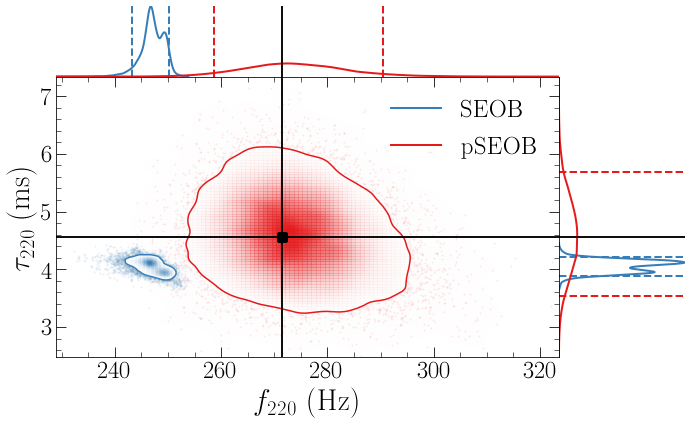
\includegraphics[width=0.5\textwidth]{figures/GW150914_simulated_signal_0p1_gr_ngr_fngrtaungr.png}
        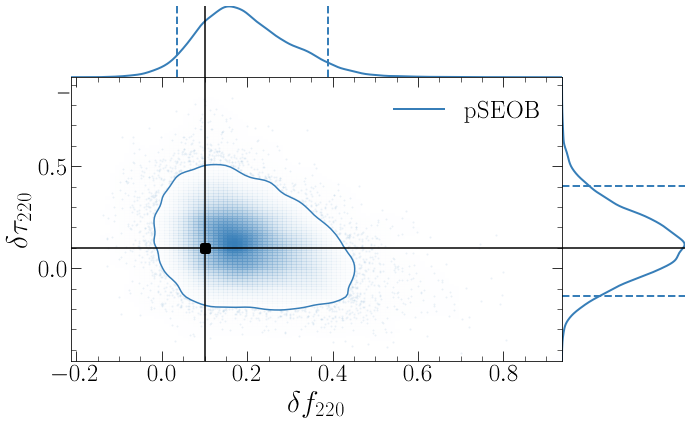
\includegraphics[width=0.5\textwidth]{figures/GW190521_simulated_signal_0p1_deltaf220_deltatau220.png}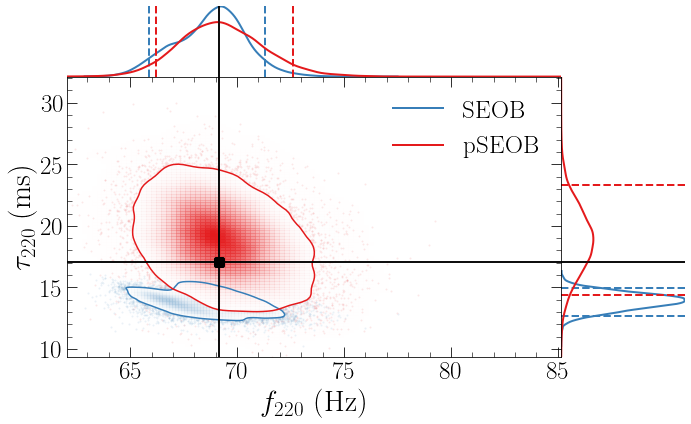
\includegraphics[width=0.5\textwidth]{figures/GW190521_simulated_signal_0p1_gr_ngr_fngrtaungr.png}
        \caption{\textcolor{red}{FINAL RESULT} Posterior probability distribution on the fractional deviations in the frequency and damping time of the $(2,2)$ QNM, $(\df{220},\dtau{220})$ (left panels) and the reconstructed quantities, $(\fngr{220}, \taungr{220})$ (right panels) for non-GR injections ($\pSEOB$) with parameters of GW150914-like (top panels) and GW190521-like (bottom panels) as given in Table~\ref{tab:injection_values}. The non-GR signal has a deviation, $\df{220} = \dtau{220} = 0.1$. The 2D contour marks the 90\% credible region, while the dashed lines on the 1D marginalized distributions mark the 90\% credible levels. The black vertical and horizontal lines mark the injection values. In the right panels, we additionally show measurements using a GR ($\SEOB$) waveform, for the
GW150914-like (upper panel) and GW190521-like (lower panel) injections. The measurements with $\SEOB$ waveforms are visibly biased.}
        \label{fig:simulated_signal_nonGR}
\end{center}
\end{figure*}
%%%%%%%%%%%%%%%%%%%%%%%%%%%%%%%%%%%%%%%%%%%%%%%%%%%%%%%%%%%%%%%
%%%%%%%%%%%%%%%%%%%%%%%%%%%%%%%%%%%%%%%%%%%%%%%%%%%%%%%%%%%%%%%

\iffalse
%%%%%%%%%%%%%%%%%%%%%%%%%%%%%%%%%%%%%%%%%%%%%%%%%%%%%%%%%%%%%%%
% modified GR signal: GR vs nonGR recovery comparison
%%%%%%%%%%%%%%%%%%%%%%%%%%%%%%%%%%%%%%%%%%%%%%%%%%%%%%%%%%%%%%%
\begin{figure*}%[h!]
        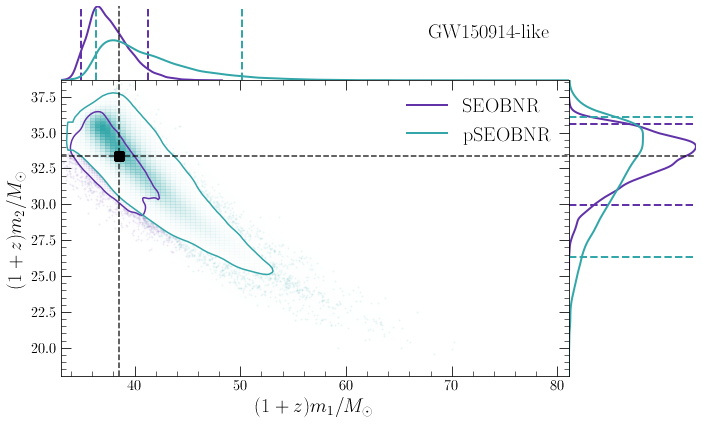
\includegraphics[width=0.5\textwidth]{figures/GW150914_simulated_signal_0p1_gr_ngr_m1m2.png}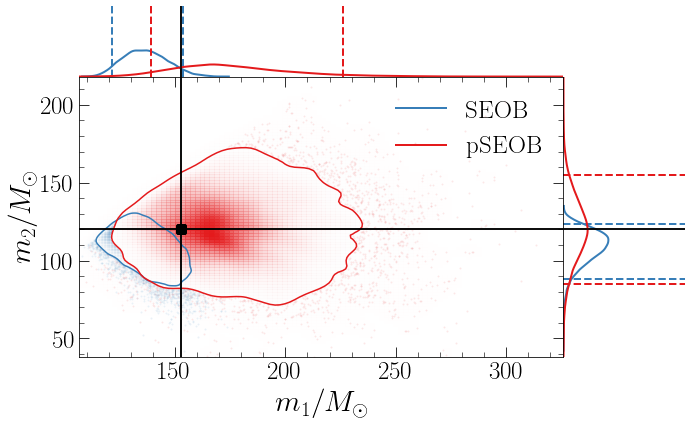
\includegraphics[width=0.5\textwidth]{figures/GW190521_simulated_signal_0p1_gr_ngr_m1m2.png}
        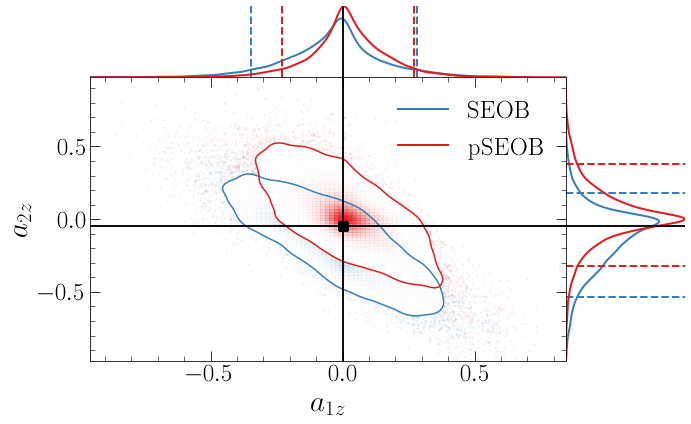
\includegraphics[width=0.5\textwidth]{figures/GW150914_simulated_signal_0p1_gr_ngr_a1za2z.png}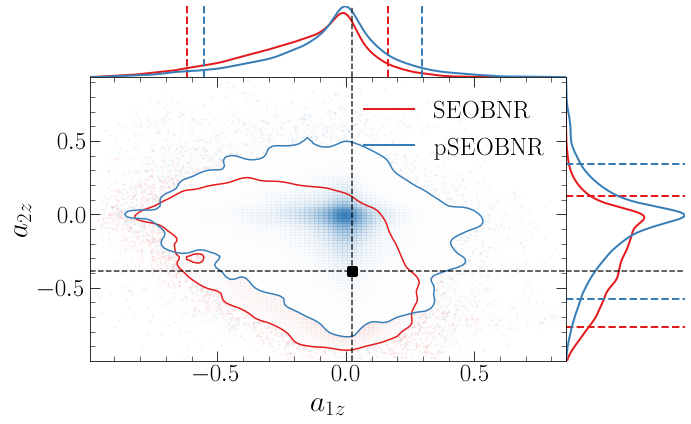
\includegraphics[width=0.5\textwidth]{figures/GW190521_simulated_signal_0p1_gr_ngr_a1za2z.png}
        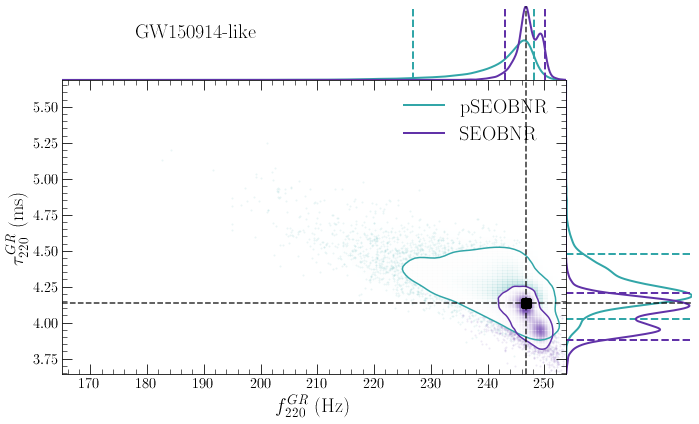
\includegraphics[width=0.5\textwidth]{figures/GW150914_simulated_signal_0p1_gr_ngr_fgrtaugr.png}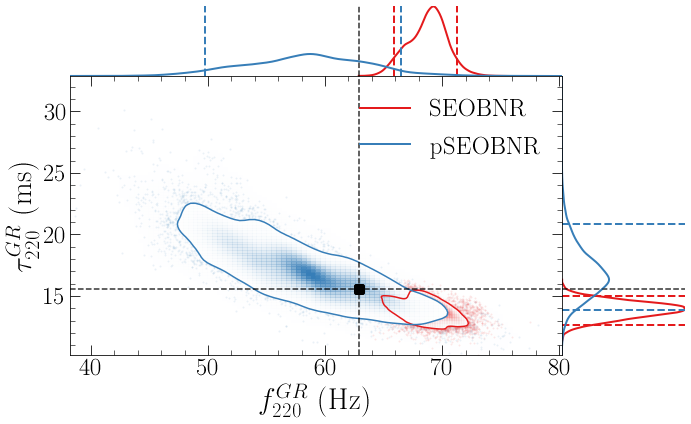
\includegraphics[width=0.5\textwidth]{figures/GW190521_simulated_signal_0p1_gr_ngr_fgrtaugr.png}
        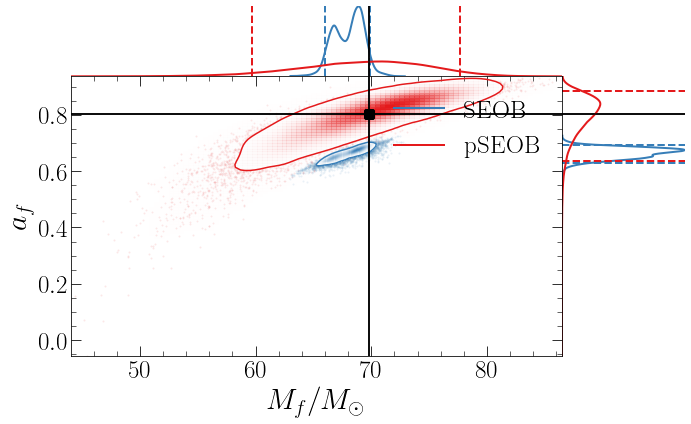
\includegraphics[width=0.5\textwidth]{figures/GW150914_simulated_signal_0p1_gr_ngr_Mfaf.png}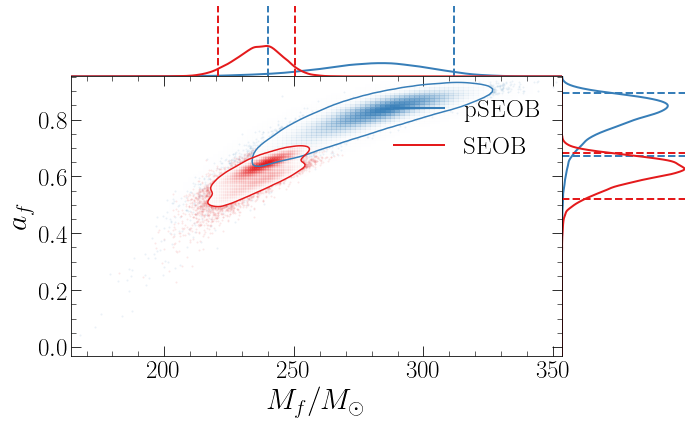
\includegraphics[width=0.5\textwidth]{figures/GW190521_simulated_signal_0p1_gr_ngr_Mfaf.png}
        \caption{\textcolor{red}{FINAL RESULT} Comparison of binary's parameters when a non-GR signal ($\pSEOB$) is injected and recovered with a GR ($\SEOB$) or a non-GR ($\pSEOB$) waveform model. The left (right) panels refer to
a GW150914-like (GW190521- like) injected signal (see Table~\ref{tab:injection_values}) with QNM deviation parameters of $\df{220} = \dtau{220} = 0.1$. The panels (from top to bottom) show the 2D posteriors (with 90\% credible levels) and corresponding marginalised 1D posteriors (with 90\% credible levels) in (detector-frame) masses (first row), dimensionless spins (second row), GR predictions of frequency and damping time (third row) and the remnant mass and spin predictions ($M_f$, $\chi_f$) from the frequency and damping time. In each case, the injection values are indicated by the black dashed lines.}
        \label{fig:gr_ngr_comparison}
\end{figure*}
%%%%%%%%%%%%%%%%%%%%%%%%%%%%%%%%%%%%%%%%%%%%%%%%%%%%%%%%%%%%%%%
%%%%%%%%%%%%%%%%%%%%%%%%%%%%%%%%%%%%%%%%%%%%%%%%%%%%%%%%%%%%%%%
\fi
%%%%%%%%%%%%%%%%%%%%%%%%%%%%%%%%%%%%%%%%%%%%%%%%%%%%%%%%%%%%%%%
% GW150914-like signal with different deviations: GR vs nonGR recovery
%%%%%%%%%%%%%%%%%%%%%%%%%%%%%%%%%%%%%%%%%%%%%%%%%%%%%%%%%%%%%%%
\begin{figure*}%[h!]
        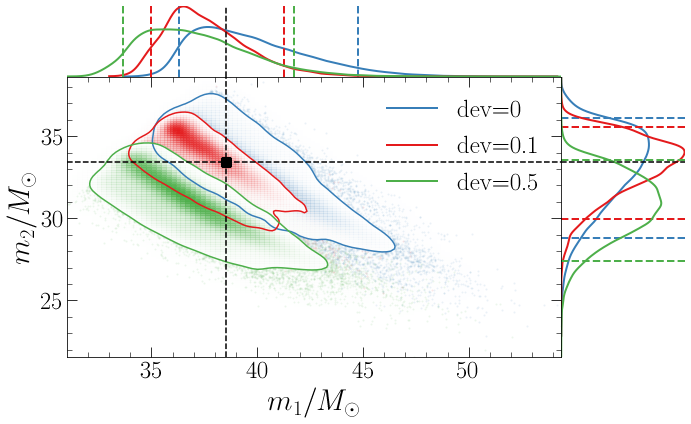
\includegraphics[width=0.5\textwidth]{figures/GW150914_simulated_signal_0p0_0p1_0p5_gr_m1m2.png}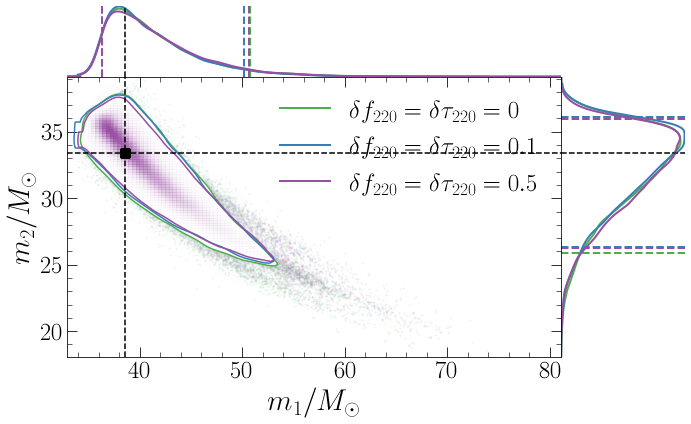
\includegraphics[width=0.5\textwidth]{figures/GW150914_simulated_signal_0p0_0p1_0p5_ngr_m1m2.png}
        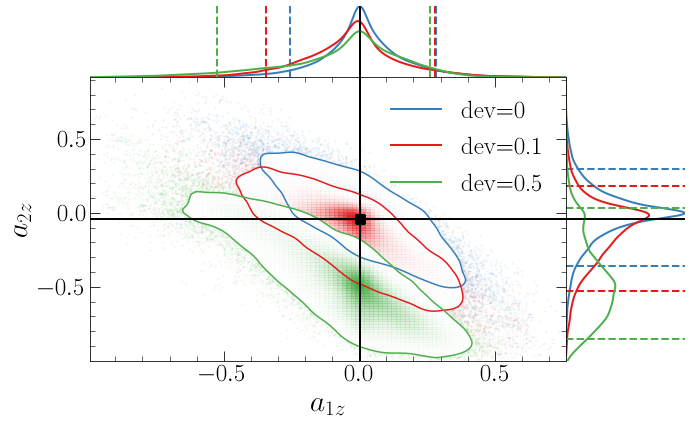
\includegraphics[width=0.5\textwidth]{figures/GW150914_simulated_signal_0p0_0p1_0p5_gr_a1za2z.png}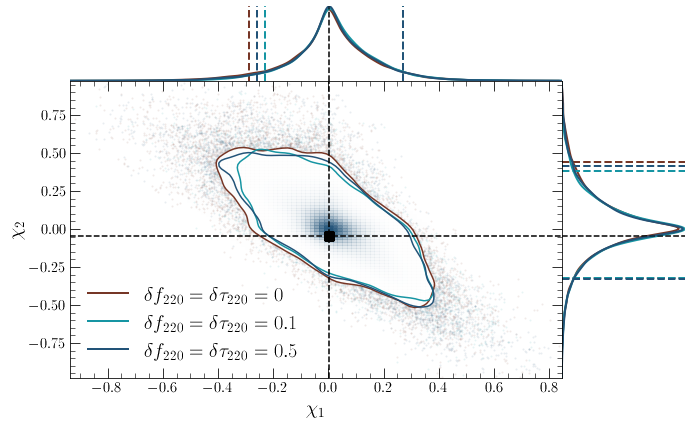
\includegraphics[width=0.5\textwidth]{figures/GW150914_simulated_signal_0p0_0p1_0p5_ngr_a1za2z.png}
        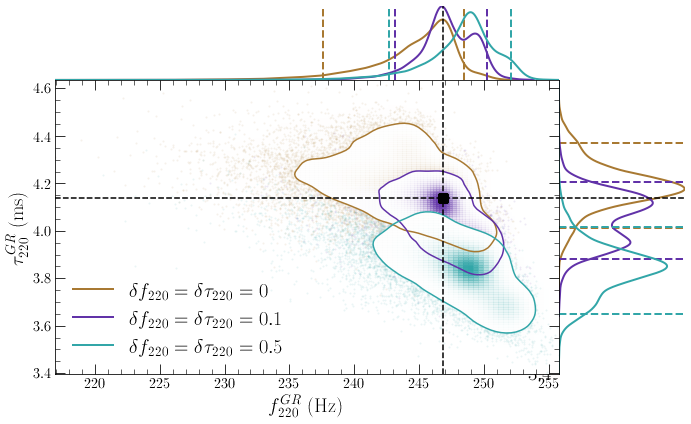
\includegraphics[width=0.5\textwidth]{figures/GW150914_simulated_signal_0p0_0p1_0p5_gr_fgrtaugr.png}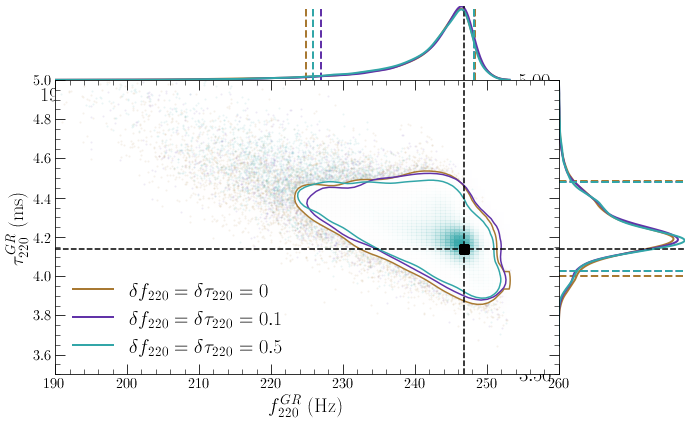
\includegraphics[width=0.5\textwidth]{figures/GW150914_simulated_signal_0p0_0p1_0p5_ngr_fgrtaugr.png}
        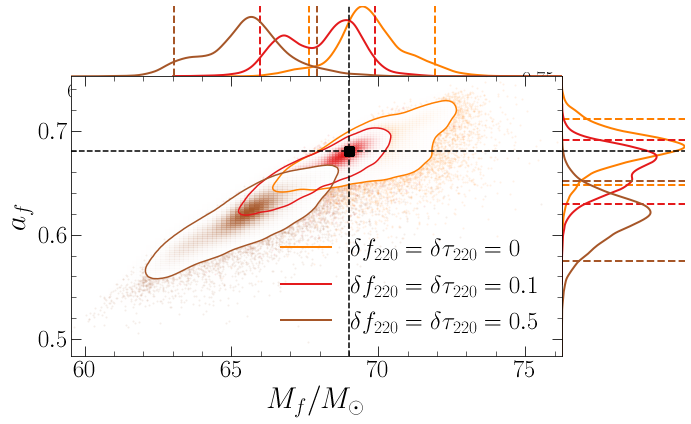
\includegraphics[width=0.5\textwidth]{figures/GW150914_simulated_signal_0p0_0p1_0p5_gr_Mfaf.png}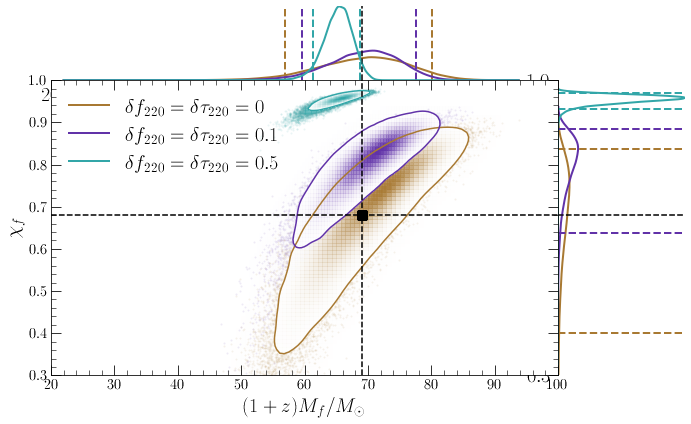
\includegraphics[width=0.5\textwidth]{figures/GW150914_simulated_signal_0p0_0p1_0p5_ngr_Mfaf.png}
        \caption{\textcolor{red}{FINAL RESULT}  Comparison of a GW150914-like injection's parameters when signals with zero, 10\% and 50\% deviations ($\df{220} = \dtau{220} = 0, 0.1, 0.5$) are recovered using a GR ($\SEOB$) (left panels) or a non-GR ($\pSEOB$) (right panels) waveform model. The panels (from top to bottom) show the 2D posteriors (with 90\% credible levels) and corresponding marginalised 1D posteriors (with 90\% credible levels) in (detector-frame) masses (first row), dimensionless spins (second row), GR predictions of frequency and damping time (third row) and the remnant mass and spin predictions ($M_f$, $\chi_f$) from the frequency and damping time. In each case, the injection values are indicated by the black dashed lines. In the lowermost panel, the injection values of the final mass and spin, correspond to the injection with no deviations. The $\df{220} = \dtau{220} = 0.1$ signal is identical to the results shown in Fig.~\ref{fig:simulated_signal_nonGR}.}
        \label{fig:gr_ngr_comparison}
\end{figure*}
%%%%%%%%%%%%%%%%%%%%%%%%%%%%%%%%%%%%%%%%%%%%%%%%%%%%%%%%%%%%%%%
%%%%%%%%%%%%%%%%%%%%%%%%%%%%%%%%%%%%%%%%%%%%%%%%%%%%%%%%%%%%%%%

We additionally investigate the effects of erroneously assuming that
an underlying non-GR signal can be well-described by a GR one. We do
this by estimating the parameters of our non-GR signals using the GR
waveform model $\SEOB$ instead of the parameterized $\pSEOB$.  The
resulting one- and two-dimensional posteriors are shown in the right
panels of Fig.~\ref{fig:simulated_signal_nonGR} by red curves for the
GW150914-like (top) and GW190521-like (bottom) signals
respectively. For both signals, we find the $\SEOB$ estimates are
markedly biased with respect to the $\pSEOB$ estimates. We also notice that the
results are distinctly different for the two events. For the
GW150914-like non-GR signal, the measurements of $(\fgr{220},
\taugr{220})$ (top right panel in
Fig.~\ref{fig:simulated_signal_nonGR}) are consistent with the
$(\fngr{220}, \taungr{220})$ measurements for a signal with \emph{no
  deviations} from GR (top right panel in
Fig.~\ref{fig:simulated_signal_GR}). In other words, if the actual
signal had deviations from GR as large as the $10\%$, the analysis
with the GR signal $\SEOB$ would likely have reported \emph{no}
deviation from the GR prediction. However in the case of the
GW190521-like non-GR signal, a simple GR analysis of the non-GR signal
would have yielded measurements distinctly different from either of
the two parameterized estimates: with and without deviations.

Finally, we investigate the impact on the estimation of the GR parameters $\bxigr$ as we change the
magnitude of deviation in the non-GR parameters. We restrict ourselves 
to a GW150914-like event, and for comparison, add a synthetic signal
with $\df{220} = \dtau{220} = 0.5$, or 50 \% deviation, alongside the
10\% non-GR signal and a signal with no deviation (essentially GR)
mentioned above. We summarise the results in
Fig.~\ref{fig:gr_ngr_comparison}. The left (right) panels show the
posterior probability distributions of the three signals using the GR,
$\SEOB$ (non-GR, $\pSEOB$) waveform model. The first difference we
note is the $\SEOB$ recoveries yield biased estimates when the
underlying signal is non-GR, while the $\pSEOB$ recoveries do
not. Furthermore, as we increase the deviations, while the $\SEOB$
recoveries expectedly get more biased, the $\pSEOB$ measurements are
robust in consistently recovering the injected value. Since the
measurement of the frequency and damping time in the $\pSEOB$ model
incorporate information from the masses and spins through the NR
fitting formulae (as shown in
Eqs.~(\ref{eq:nongr_freqs_a})---(\ref{eq:nongr_freqs_b})), one might have
expected correlations between the mass, spins and the QNM frequencies,
leading to biased estimates in the masses and spins. We confirm here
that is not the case. \comment{AB: I don't see how from the figure I can  
conclude that there are no correlations between masses/spins and QNMs.}






\subsection{Test of the no-hair conjecture}\label{ssec:nohairtheorem}

Finally, we provide a simple demonstration of a test of the no-hair
theorem using our model. As described in the introduction, any test of
the no-hair theorem of BHs would need to involve independent
measurements of (at least) two different QNMs.

Here, we use an NR GW signal from the SXS catalog~\cite{Mroue:2013xna}
corresponding to a non-spinning BBH with mass-ratio $q=6$ (SXS:BBH:0166) and 
total mass $M=84 \Mo$ (see Table~\ref{tab:injection_values}).
We choose an asymmetric system to increase the SNR in the higher modes.
We also choose the distance and orientation of the binary
such that the total SNR in the three-detector network of LIGO Hanford, Livingston and
Virgo, is \macro{$\sim$ 70}. Based on the LIGO-Virgo observations during the first three observing runs, 
such asymmetric and loud signals are no longer just a theoretical
prediction, but quite plausible during O4. Using this
signal, we attempt to measure both the $(2,2)$ and
$(3,3)$ QNMs. For this injected signal the SNR in
other sub-dominant modes is too low to be able to measure them.

We summarize our results in Fig.~\ref{fig:nohair_sxs}.  Given the
injection parameters, the predicted values of the $(2, 2)$ and
$(3, 3)$ frequency and damping time are \macro{(169.45 Hz, 4.68
  ms)} and \macro{(271.21 Hz, 4.50 ms)} respectively. The left panel
of Fig.~\ref{fig:nohair_sxs} shows that the 2D posteriors
on the $(2, 2)$ and $(3, 3)$ QNMs are consistent with the
predictions for a BBH merger in GR, indicated by the black plus sign.
Using fitting formulae provided in Ref.~\cite{Berti:2005ys}, specifically,
Eq.~(2.1), Eq.~(E1) and Eq.~(E3) and Tables VIII and IX for the fitting coefficients,
we infer the 2D posterior probability distribution on the
final mass and spin for the $(2, 2)$ (blue) and $(3, 3)$ (red)
QNMs in the right panel of Fig.~\ref{fig:nohair_sxs}. The two
independent estimates are consistent with each other and correspond to
a unique mass and spin for the remnant BH \macro{(83.08 $\Mo$, 0.37)}
indicated by the plus sign. As a consequence, this may be considered
as a test of the no-hair conjecture. For most of the events observed
so far, the power in the $(3, 3)$ has not been sufficient to
measure it along with the $(2, 2)$, or in fact, in its
place. However, it might also be possible to combine information from
multiple observation over the coming few years to obtain meaningful
constraints on the $(3, 3)$ and other sub-dominant QNMs.

%%%%%%%%%%%%%%%%%%%%%%%%%%%%%%%%%%%%%%%%%%%%%%%%%%%%%%%%%%%%%%%

%%%%%%%%%%%%%%%%%%%%%%%%%%%%%%%%%%%%%%%%%%%%%%%%%%%%%%%%%%%%%%%
\begin{figure}
        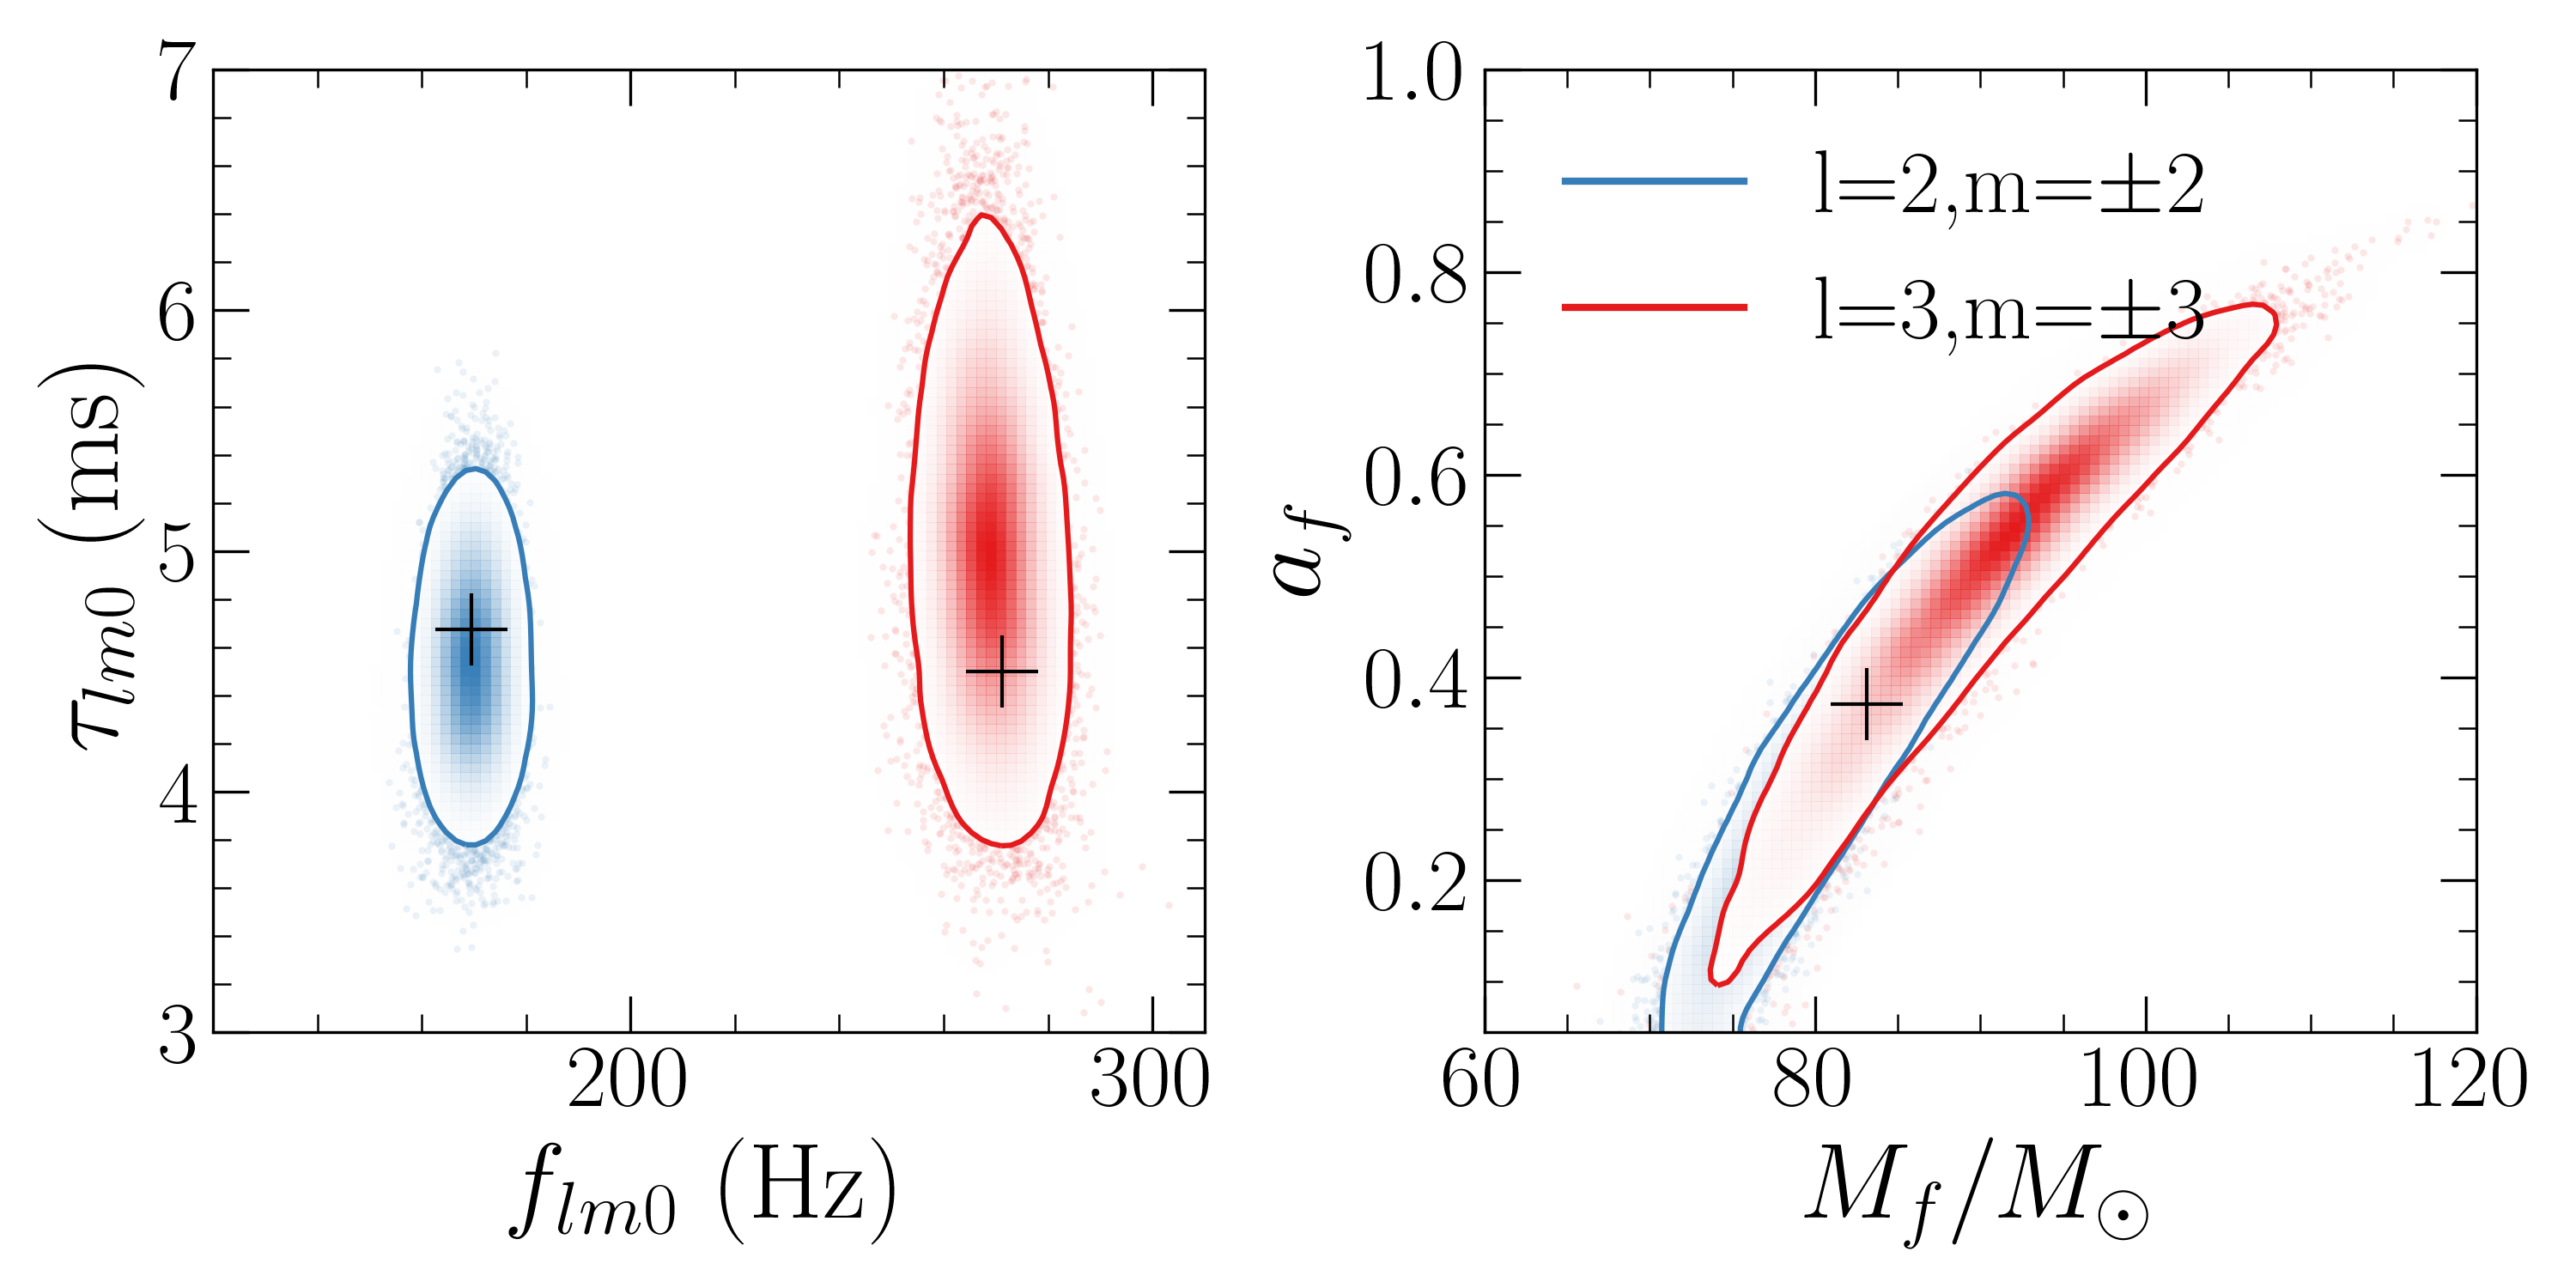
\includegraphics[width=0.5\textwidth]{figures/nohair_sxs_0166.png}
        \caption{\textcolor{red}{FINAL RESULT} Posterior probability distribution on the frequency and damping time of the $(2, 2)$ and $(3, 3)$ QNM (left panel), and the final mass and spin inferred from the complex frequencies (right panel), when a NR signal with parameters $q=6$,  $M=84 \Mo$ and SNR $=75$ is injected in Gaussian noise and recovered with the $\pSEOB$ waveform model. The plus signs mark the GR predictions.}
        \label{fig:nohair_sxs}
\end{figure}
%%%%%%%%%%%%%%%%%%%%%%%%%%%%%%%%%%%%%%%%%%%%%%%%%%%%%%%%%%%%%%%
%%%%%%%%%%%%%%%%%%%%%%%%%%%%%%%%%%%%%%%%%%%%%%%%%%%%%%%%%%%%%%%
